\chapter{Propuesta de solución}\label{chapter:solution_proposal}

En este capítulo se plantea una forma de obtener, a partir de un conjunto de datos de la forma $\{(t_i, y_i), y \in \mathbb{R}^n, i = 1, \dots, K\}$, un sistema de $n$ ecuaciones diferenciales lineales con respecto a los parámetros que mejor los describa. El sistema se obtiene mediante el uso de la regresión simbólica utilizando un algoritmo genético. Para determinar cuán bien un sistema de ecuaciones diferenciales dado, describe al conjunto de datos, se resuelve un problema de mínimos cuadrados para estimar los mejores parámetros.

La sección \ref{section:solution_representation} detalla cómo se puede representar un sistema de EDOs lineales en los parámetros mediante un árbol computacional. En \ref{section:solution_cost} se explica la función de ajuste que se tiene en cuenta en la regresión simbólica planteada. En las secciones \ref{section:mutation}, \ref{section:xcross} y \ref{section:selection} se detallan las operaciones necesarias para la aplicación de un algoritmo genético: la mutación, el cruzamiento y la selección, respectivamente. A continuación se describe cómo representar sistemas de ecuaciones linales mediante árboles computacionales.


\section{Representación de Sistemas de EDOs mediante árboles}\label{section:solution_representation}

A partir de datos de la forma $\{(t_i, y_i), y \in \mathbb{R}^n, i = 1, \dots, K\}$, se puede determinar la cantidad de ecuaciones que posee el sistema: una por cada dimensión que tenga el vector $y$. Por ejemplo, si cada elemento de los datos es de la forma:
$$(t_i, y_{1_i}, \dots, y_{n_i}),$$
entonces se tiene la certeza de que el sistema de ecuaciones diferenciales que se desea tiene $n$ ecuaciones, y que los sistemas de ecuaciones en el espacio de búsqueda del método deben tener la forma:
$$y_1' = f_1(t, y_1, \dots, y_n)$$
$$\vdots$$
$$y_n' = f_n(t, y_1, \dots, y_n)$$

Como el sistema debe tener $n$ ecuaciones, una forma de representar las soluciones candidatas es mediante una lista de $n$ elementos. La posición $i$ de la lista representa la función $f_i(t,y_1, \dots, y_n)$.

Por ejemplo, el modelo poblacional SIR:
\begin{align*}
    S' & = - aIS    \\
    I' & = aIS - bI \\
    R' & = bI,
\end{align*}
Se puede representar con la lista:
$$[-aIS, aIS - bI, bI],$$
donde los elementos de la lista están separados por coma.

Una expresión aritmética (como cada una de las posibles funciones) se puede representar mediante un árbol, donde los nodos interiores son operadores y las hojas son variables. Entonces, en la posición $i$ de la lista, se puede representar el árbol computacional que describe la parte de la derecha de la ecuación diferencial correspondiente a la ecuación $i$.

Sin embargo, con la representación descrita por Koza \cite{zelinka2005analytic}, no se plantea de forma explícita la linealidad de las ecuaciones diferenciales con respecto a los parámetros. Esta linealidad es importante dado que el sistema que se busca como solución debe cumplir esta propiedad. En este trabajo se modifica la estructura del árbol para garantizar que todos los árboles representen sistemas de ecuaciones diferenciales lineales con respecto a los parámetros.

Como la parte derecha de una ecuación diferencial lineal con respecto a los parámetros es una suma de multiplicaciones de parámetros con funciones que no dependen de parámetros:
$$\frac{dX_i}{dt} = \sum_{i=1}^{n} a_i * f_i(t, y(t)),$$
entonces cada una de las partes derechas de las ecuaciones diferenciales se representan con un árbol en el que la raíz es un nodo con una operación especial de suma, que puede tener cualquier cantidad de sumandos (o de hijos) como se muestra en la figura \ref{tikzpicture:doe_node_example}.

% \begin{center}
%     \begin{tikzpicture}[
%             roundnode/.style={circle, draw, fill=gray!25, very thick, minimum size=7mm},
%             roundnode_transparent/.style={circle, very thick, minimum size=5mm}
%         ]
%         % Nodes
%         \node[roundnode]        (plus)                            {$+$};
%         \node[roundnode]        (term_1)     [below left=of plus]        {$a_1 * f_1(t, y(t))$};
%         \node[roundnode_transparent]        (term_dots)     [below =of plus]        {$\dots$};
%         \node[roundnode]        (term_n)     [below right=of plus]        {$a_n * f_n(t, y(t))$};


%         %Lines
%         \draw [->] (plus.south) -- (term_1.north);
%         % \draw [->] (plus.south) -- (term_dots.north);
%         \draw [->] (plus.south) -- (term_n.north);
%     \end{tikzpicture}
% \end{center}

\begin{figure}[h]
    \centering
    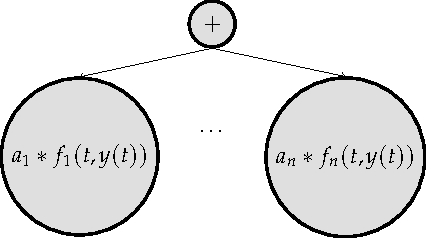
\includegraphics[width=0.5\textwidth]{"figures/doe_node_example.pdf"}
    \caption{Estructura del árbol de una ecuación diferencial lineal en los parámetros.}
    \label{tikzpicture:doe_node_example}
\end{figure}

Cada uno de los hijos del nodo que representa la parte derecha de una ecuación diferencial es un subárbol que representa la multiplicación de un parámetro con una función que no depende de parámetros.

Estos subárboles poseen como raíz un nodo con una operación de multiplicación y dos nodos hijos. El primero de ellos es un nodo hoja que representa el parámetro. El segundo hijo es un nodo que representa el subárbol computacional correspondiente a la función, utilizando la misma representación que plantea Koza \cite{zelinka2005analytic} pero con la peculiaridad de que sus hojas solo podrán almacenar variables, no parámetros. La figura \ref{tikzpicture:doe_term_node_example} muestra la estructura del subárbol que representa la multiplicación de un parámetro con una función que no depende de parámetros.

% \begin{center}
%     \begin{tikzpicture}[
%             roundnode/.style={circle, draw, fill=gray!25, very thick, minimum size=7mm},
%             squarednode/.style={rectangle, draw, fill=gray!25, very thick, minimum size=7mm}
%         ]
%         % Nodes
%         \node[roundnode]        (star)                            {$*$};
%         \node[squarednode]        (term_1)     [below left=of star]        {$a_i$};
%         \node[roundnode]        (term_n)     [below right=of star]        {$f_i(t, y(t))$};


%         %Lines
%         \draw [->] (star.south) -- (term_1.north);
%         \draw [->] (star.south) -- (term_n.north);
%     \end{tikzpicture}
% \end{center}

\begin{figure}[h]
    \centering
    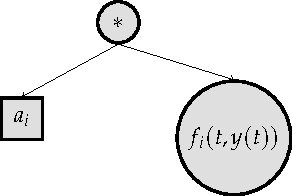
\includegraphics[width=0.5\textwidth]{"figures/doe_term_node_example.pdf"}
    \caption{Estructura del árbol de un término perteneciente a una ecuación diferencial lineal en los parámetros.}
    \label{tikzpicture:doe_term_node_example}
\end{figure}


Un sistema de ecuaciones diferenciales se puede representar como un árbol donde cada ecuación sea un hijo. Como ejemplo se puede utilizar el modelo poblacional SIR, que es lineal con respecto a sus parámetros, y su representación con la estructura propuesta sería la que se muestra en la figura \ref{tikzpicture:sir_example}.

% \begin{center}
%     \begin{tikzpicture}[
%             roundnode/.style={circle, draw, fill=gray!25, very thick, minimum size=7mm},
%             squarednode/.style={rectangle, draw, fill=gray!25, very thick, minimum size=5mm}
%         ]
%         % Nodes
%         \node[roundnode]        (system)                            {$SYSTEM$};

%         \node[roundnode]        (plus_S)     [below left=of system]        {$+$};
%         \node[roundnode]        (star_S_1)    [below left=of plus_S]    {$*$};
%         \node[squarednode]      (alpha_star_S_1)      [below left=of star_S_1]    {$a$};
%         \node[roundnode]        (neg_star_S_1)    [below=of star_S_1]    {$-$};
%         \node[roundnode]        (star_S_2)    [below=of neg_star_S_1]    {$*$};
%         \node[squarednode]      (S_star_S)       [below left=of star_S_2]   {$S$};
%         \node[squarednode]      (I_star_S)      [below=of star_S_2]   {$I$};

%         \node[roundnode]        (plus_I)     [below=of system]        {$+$};
%         \node[roundnode]        (star_I_1)    [below left=of plus_I]    {$*$};
%         \node[squarednode]      (alpha_star_I_1)      [below left=1cm and 0.5cm of star_I_1]    {$a$};
%         \node[roundnode]        (star_I_2)    [below=of star_I_1]    {$*$};
%         \node[squarednode]      (S_star_I)       [below left=1cm and 0.5cm of star_I_2]   {$S$};
%         \node[squarednode]      (I_star_I_1)      [below=of star_I_2]   {$I$};

%         \node[roundnode]        (star_I_3)    [below right=of plus_I]    {$*$};
%         \node[squarednode]      (beta_star_I_1)      [below=of star_I_3]    {$b$};
%         \node[roundnode]        (neg_star_I_1)    [below right=1cm and 0.5cm of star_I_3]    {$-$};
%         \node[squarednode]      (I_star_I_2)      [below=of neg_star_I_1]   {$I$};

%         \node[roundnode]        (plus_R)     [below right=of system]        {$+$};
%         \node[roundnode]        (star_R_1)    [below right=of plus_R]    {$*$};
%         \node[squarednode]      (beta_star_R_1)      [below=of star_R_1]    {$b$};
%         \node[squarednode]      (I_star_R)      [below right=of star_R_1]   {$I$};

%         %Lines
%         \draw [->] (system.south) -- (plus_S.north);
%         \draw[->] (system.south) -- (plus_I.north);
%         \draw[->] (system.south) -- (plus_R.north);

%         \draw[->] (plus_S.south) -- (star_S_1.north);
%         \draw[->] (star_S_1.south) -- (alpha_star_S_1.north);
%         \draw[->] (star_S_1.south) -- (neg_star_S_1.north);
%         \draw[->] (neg_star_S_1.south) -- (star_S_2.north);
%         \draw[->] (star_S_2.south) -- (S_star_S.north);
%         \draw[->] (star_S_2.south) -- (I_star_S.north);

%         \draw[->] (plus_I.south) -- (star_I_1.north);
%         \draw[->] (plus_I.south) -- (star_I_3.north);
%         \draw[->] (star_I_1.south) -- (alpha_star_I_1.north);
%         \draw[->] (star_I_1.south) -- (star_I_2.north);
%         \draw[->] (star_I_2.south) -- (S_star_I.north);
%         \draw[->] (star_I_2.south) -- (I_star_I_1.north);

%         \draw[->] (star_I_3.south) -- (beta_star_I_1.north);
%         \draw[->] (star_I_3.south) -- (neg_star_I_1.north);
%         \draw[->] (neg_star_I_1.south) -- (I_star_I_2.north);

%         \draw[->] (plus_R.south) -- (star_R_1.north);
%         \draw[->] (star_R_1.south) -- (beta_star_R_1.north);
%         \draw[->] (star_R_1.south) -- (I_star_R.north);
%     \end{tikzpicture}
% \end{center}

\begin{figure}[h]
    \centering
    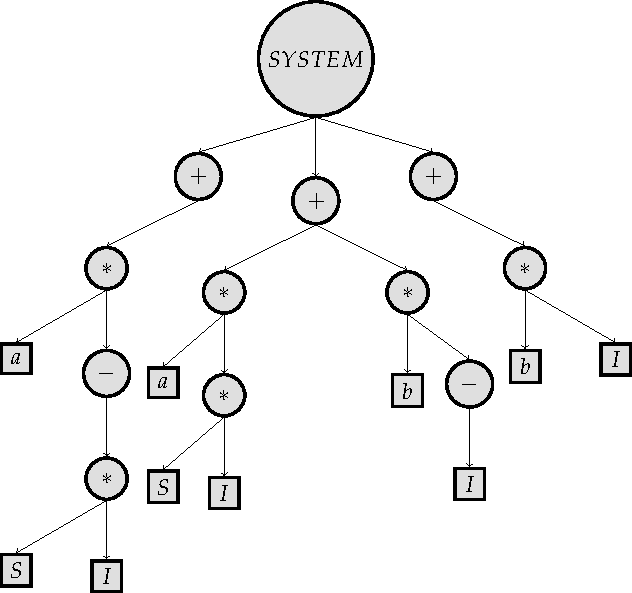
\includegraphics[width=0.5\textwidth]{"figures/sir_example.pdf"}
    \caption{Estructura del árbol que representa el modelo poblacional SIR.}
    \label{tikzpicture:sir_example}
\end{figure}

Con esta representación se pueden expresar todos los sistemas de ecuaciones diferenciales lineales con respecto a los parámetros en los que intervengan un conjunto de operaciones prefijadas de antemano, que son los posibles nodos interiores. Esta representación se utiliza en los modelos que se generan en el algoritmo de regresión simbólica que se detalla en la secciones \ref{section:mutation} y \ref{section:xcross}.

En un método de regresión simbólica es necesario tener una función de ajuste que permita conocer cuán cercanos son los datos predichos por el modelo a los datos observados. En la siguiente sección se propone un método para evaluar cuán cercanos se encuentran los datos predichos y los observados.

\section{Determinar el costo de una solución}\label{section:solution_cost}

A partir de un conjunto de datos:
$$M = \{(t_j, y_i(t_j)), i = 1, \dots, n, j = 1, \dots, m\},$$
donde la función $y_i$ es desconocida, se puede aproximar el valor de las derivadas de $y_i$ en cada instante $t_j$ utilizando el método de diferencias finitas \cite{gaucel2014learning}, en caso de que $M$ no posea ruido. Si el conjunto de datos $M$ tiene ruido se puede aproximar la función $y_i$ mediante un spline de suavizado cúbico. Con la expresión de este spline de suavizado se puede obtener una aproximación del valor de la derivada de la función $y_i$ en cada instante $t_j$.

Luego de aproximar la derivada de las funciones $y_i$ en cada instante $t_j$ se puede generar un nuevo conjunto de la forma:
$$\{(t_j, y_i(t_j), y'_{i}(t_j)), i = 1, \dots, n, j = 1, \dots, m\},$$
donde $y'_{i}(t_j)$ es el valor de la aproximación de la derivada de la función $y_i$ en el instante $t_j$.

Por ejemplo, si se tienen el conjunto de datos sin ruido:
\begin{align*}
    \{ & (1, 1)     \\
       & (2, 4)     \\
       & (3, 9) \},
\end{align*}
y se desea conocer el valor aproximado de la derivada de la función $y$ en los instantes $1$ y $2$ se puede utilizar el método de diferencias finitas para obtener los datos:
\begin{align*}
    y'(1) & = \frac{y(2) - y(1)}{2 - 1} = 3  \\
    y'(2) & = \frac{y(3) - y(2)}{3 - 2} = 5.
\end{align*}

Con esta aproximación de la derivada se puede formar el nuevo conjunto de datos:
\begin{align*}
    \{ & (1, (1), (3))    \\
       & (2, (4), (5)) \}
\end{align*}

Se define el costo de un sistema de ecuaciones diferenciales $f$ para el conjunto de datos de la forma:
$$\{(t_j, y_i(t_j), y'_i(t_j)) \subset \mathbb{R} \times \mathbb{R}^{n} \times \mathbb{R}^n, i = 1, \dots, n, j = 1, \dots, m\}$$
como:
$$C = \frac{\sum_{i=1}^n\frac{\sum_{j=1}^{m}(y'_i(t_j) - f_i(t_j, y_i(t_j)))^2}{m}}{n},$$
donde:
$$f_i(t_j, y_i(t_j)) = \sum_{k=1}^{p_i} a_{i_k} * g_{i_k}(t_j, y_i(t_j)),$$
$f_1(t_j, y_i(t_j)), f_2(t_j, y_i(t_j)), \dots, f_n(t_j, y_i(t_j))$ son las partes derechas de las ecuaciones del sistema y $p_i$ indica la cantidad de parámetros presentes en la ecuación $i$ del sistema. Mientras más pequeño es el valor del costo, mejor se describen los datos mediante el sistema $f$.

Al valor de $C$ se le agrega un factor de peso $P$, directamente proporcional a la cantidad de términos que posean las ecuaciones de la solución \cite{gplearnbloat}:
$$P = \begin{cases}
        Constant * node\_count(f), & \text{si } node\_count(f) \geq MAX\_NODES \\
        0,                         & \text{en otro caso}
    \end{cases}.$$

$Node\_count(f)$ es la cantidad de nodos presentes en la representación en forma de árbol computacional del sistema $f$. $Constant$ es una constante definida en la implementación y en los experimentos realizados en el capítulo \ref{chapter:results} se utiliza un valor de 9999.

El parámetro $MAX\_NODES$ se define junto con los demás parámetros del algoritmo genético y en los experimentos del capítulo \ref{chapter:results} se usaron valores entre 15 y 40. El factor de peso garantiza que si dos ecuaciones son capaces de generar los mismos puntos, la ecuación con menos términos tenga una mejor evaluación en la función objetivo.

Para que la suma $\sum_{j=1}^{m}(y'_{i_j} - f_i(x_j)) ^ 2$ sea la menor posible se debe minimizar la diferencia $(y'_{i_j} - f_i(x_j))^2$, y para ello que se crea, por cada ecuación del sistema, un sistema de ecuaciones de la forma $A_i * x_i = B_i$ donde:
\begin{align*}
    A_i & = \begin{pmatrix}
        g_{i_1}(x_1) & g_{i_2}(x_1) & \dots  & g_{i_k}(x_1) \\
        g_{i_1}(x_2) & g_{i_2}(x_2) &        & g_{i_k}(x_2) \\
        \vdots       & \vdots       & \ddots & \vdots       \\
        g_{i_1}(x_m) & g_{i_2}(x_m) &        & g_{i_k}(x_m)
    \end{pmatrix}
    \qquad
    x_i = \begin{bmatrix}
        a_{i_1} \\
        a_{i_2} \\
        \vdots  \\
        a_{i_k}
    \end{bmatrix}
    \qquad
    B_i = \begin{bmatrix}
        y'_{i_1} \\
        y'_{i_2} \\
        \vdots   \\
        y'_{i_m}
    \end{bmatrix}.
\end{align*}

El sistema $A_ix_i = B_i$ se resuelve usando el comando:

\texttt{numpy.linalg.lstsq},

que emplea la descomposición SVD \cite{numpy-lstsq}.

Por ejemplo, la segunda ecuación del modelo SIR es:
$$f_I (t,S,I,R) = a_{I_1} * I * S + a_{I_2} * -I.$$
Si se tiene el conjunto de datos de la forma:
$$\{(t_j, y_i(t_j), y'_i(t_j)) \subset \mathbb{R} \times \mathbb{R}^{3} \times \mathbb{R}^3, j = 1, \dots, 6\},$$
donde $y_i(t_j)$ representa los valores de $(S(t_j), I(t_j), R(T_j))$ y $y'_j$ representa los valores aproximados de $(S'(t_j), I'(t_j), R'(t_j))$:
\begin{align*}
    \{  (0.0 & , \quad (0.7, \; 0.3, \; 0.0), \quad (-0.0636, \; 0.0333, \; 0.0303))              \\
    (0.066   & , \quad (0.6958, \; 0.3022, \; 0.002), \quad (-0.0621, \; 0.0318, \; 0.0303))      \\
    (0.132   & , \quad (0.6917, \; 0.3043, \; 0.004), \quad (-0.0636, \; 0.0333, \; 0.0303))      \\
    (0.198   & , \quad (0.6875, \; 0.3065, \; 0.006), \quad (-0.0636, \; 0.0318, \; 0.0303))      \\
    (0.264   & , \quad (0.6833, \; 0.3086, \; 0.008), \quad (-0.0621, \; 0.0333, \; 0.0318))      \\
    (0.33    & , \quad (0.6792, \; 0.3108, \; 0.0101), \quad (-0.0636, \; 0.0318, \; 0.0303)) \},
\end{align*}
entonces se puede encontrar los valores de $a_1$ y $a_2$ que mejor ajusten los datos descritos formando el sistema de ecuaciones:
\begin{align*}
    A_I & = \begin{pmatrix}
        0.21   & -0.3    \\
        0.2103 & -0.3022 \\
        0.2105 & -0.3043 \\
        0.2107 & -0.3065 \\
        0.2109 & -0.3086 \\
        0.2111 & -0.3108 \\
    \end{pmatrix}
    \qquad
    x_I = \begin{bmatrix}
        a_{I_1} \\
        a_{I_2}
    \end{bmatrix}
    \qquad
    B_I = \begin{bmatrix}
        0.0333 \\
        0.0318 \\
        0.0333 \\
        0.0318 \\
        0.0333 \\
        0.0318 \\
    \end{bmatrix}.
\end{align*}

Al resolver el sistema de ecuaciones sobredeterminado se obtienen los parámetros $a_{I_1}$ = 0.28272349 y $a_{I_2}$ = 0.08836571. Este método se aplica para encontrar los parámetros de cada una de las ecuaciones del sistema y así se obtienen todos los parámetros del sistema.

Como se mencionó al inicio del capítulo, la propuesta de solución utiliza el método de regresión simbólica mediante el uso de un algoritmo genético para encontrar el sistema que mejor ajuste un conjunto de puntos. Para usar el algoritmo genético es necesario definir las operaciones de mutación, cruzamiento y selección. En la siguiente sección se describe la operación de mutación.

\section{Mutación}\label{section:mutation}

La operación de mutación genera un nuevo sistema de ecuaciones diferenciales a partir de otro existente. Esta operación selecciona el subárbol representante de una de las ecuaciones en el sistema y luego se realiza una de las siguientes modificaciones:

\begin{itemize}
    \item Eliminar un término (sumando de la ecuación) de la ecuación. Si se toman los sumandos de la ecuación como una lista de términos, el criterio consiste en seleccionar un término y eliminarlo.

          Por ejemplo, si se tiene la ecuación:
          $$a_1 * y_1 + a_2 * -(y_1 * y_2),$$
          la lista de términos correspondientes sería:
          $$[a_1*y_1, a_2 * -(y_1 * y_2)].$$

          Si se selecciona eliminar el segundo término, la lista de términos correspondiente a la ecuación resultaría:
          $$[a_1 * y_1],$$
          y la ecuación resultante sería:
          $$a_1 * y_1.$$

          El ejemplo en forma de árbol computacional se muestra en la figura \ref{tikzpicture:mutation_delete_term}.

          \begin{center}
              %   \begin{adjustbox}{width=0.35\textwidth, keepaspectratio}
              %       \begin{tikzpicture}[
              %               roundnode_dashed/.style={circle, draw, dashed, fill=gray!25, very thick, minimum size=7mm},
              %               roundnode/.style={circle, draw, fill=gray!25, very thick, minimum size=7mm},
              %               squarednode/.style={rectangle, draw, fill=gray!25, very thick, minimum size=5mm},
              %           ]
              %           %Nodes
              %           \node[roundnode]      (plus)                             {$+$};
              %           \node[roundnode]           (star1)   [below left=of plus]    {$*$};
              %           \node[squarednode]         (a_1)   [below left=of star1]    {$a_1$};
              %           \node[squarednode]         (y_1)     [below=of star1]         {$y_1$};
              %           \node[roundnode_dashed]           (star2)   [below right=of plus]   {$*$};
              %           \node[squarednode]         (a_2)    [below left=of star2]    {$a_2$};
              %           \node[roundnode]           (neg)     [below=of star2]         {$-$};
              %           \node[roundnode]           (star3)   [below=of neg]         {$*$};
              %           \node[squarednode]         (y_1_2)   [below=of star3]   {$y_1$};
              %           \node[squarednode]         (y_2)     [below right=of star3]   {$y_2$};

              %           %Lines
              %           \draw[->] (plus.south) -- (star1.north);
              %           \draw[->] (plus.south) -- (star2.north);
              %           \draw[->] (star1.south) -- (a_1.north);
              %           \draw[->] (star1.south) -- (y_1.north);
              %           \draw[->] (star2.south) -- (a_2.north);
              %           \draw[->] (star2.south) -- (neg.north);
              %           \draw[->] (neg.south) -- (star3.north);
              %           \draw[->] (star3.south) -- (y_1_2.north);
              %           \draw[->] (star3.south) -- (y_2.north);
              %       \end{tikzpicture}%
              %   \end{adjustbox}

              %   \qquad

              %   \begin{adjustbox}{width=0.20\textwidth, keepaspectratio}
              %       \begin{tikzpicture}[
              %               roundnode_dashed/.style={circle, draw, dashed, fill=gray!25, very thick, minimum size=7mm},
              %               roundnode/.style={circle, draw, fill=gray!25, very thick, minimum size=7mm},
              %               squarednode/.style={rectangle, draw, fill=gray!25, very thick, minimum size=5mm},
              %           ]
              %           %Nodes
              %           \node[roundnode]      (plus)                             {$+$};
              %           \node[roundnode]           (star1)   [below =of plus]    {$*$};
              %           \node[squarednode]         (a_1)   [below left=of star1]    {$a_1$};
              %           \node[squarednode]         (y_1)     [below right=of star1]         {$y_1$};

              %           %Lines
              %           \draw[->] (plus.south) -- (star1.north);
              %           \draw[->] (star1.south) -- (a_1.north);
              %           \draw[->] (star1.south) -- (y_1.north);
              %       \end{tikzpicture}%
              %   \end{adjustbox}

              \begin{figure}[h]
                  \centering
                  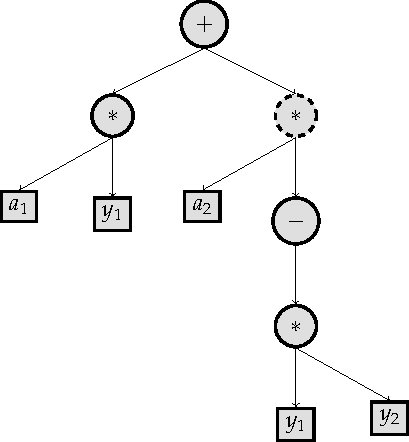
\includegraphics[width=0.3\textwidth]{"figures/mutation_delete_term_1.pdf"}
                  \qquad
                  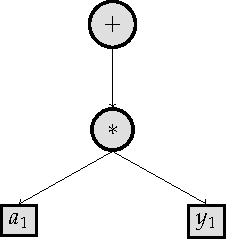
\includegraphics[width=0.3\textwidth]{"figures/mutation_delete_term_2.pdf"}
                  \caption{Ejemplo de mutación mediante la eliminación de un término en una ecuación.}
                  \label{tikzpicture:mutation_delete_term}
              \end{figure}
          \end{center}

    \item Añadir un término a la ecuación. Si se toman los sumandos de la ecuación como una lista de términos, el criterio consiste en crear un término y añadirlo.

          Por ejemplo, si se tiene la ecuación:
          $$a_1 * y_1,$$
          la lista de términos correspondientes sería:
          $$[a_1*y_1].$$

          Si se selecciona añadir como segundo sumando el término $a_2 * y_2$, la lista de términos correspondiente a la ecuación resultaría:
          $$[a_1*y_1, a_2 * y_2],$$
          y la ecuación resultante sería:
          $$a_1 * y_1 + a_2 * y_2.$$

          El ejemplo en forma de árbol computacional se muestra en la figura \ref{tikzpicture:mutation_add_term}.

          \begin{center}
              %   \begin{adjustbox}{width=0.25\textwidth, keepaspectratio}
              %       \begin{tikzpicture}[
              %               roundnode_dashed/.style={circle, draw, dashed, fill=gray!25, very thick, minimum size=7mm},
              %               roundnode/.style={circle, draw, fill=gray!25, very thick, minimum size=7mm},
              %               squarednode/.style={rectangle, draw, fill=gray!25, very thick, minimum size=5mm},
              %           ]
              %           %Nodes
              %           \node[roundnode]      (plus)                             {$+$};
              %           \node[roundnode]           (star1)   [below =of plus]    {$*$};
              %           \node[squarednode]         (a_1)   [below left=of star1]    {$a_1$};
              %           \node[squarednode]         (y_1)     [below right=of star1]         {$y_1$};

              %           %Lines
              %           \draw[->] (plus.south) -- (star1.north);
              %           \draw[->] (star1.south) -- (a_1.north);
              %           \draw[->] (star1.south) -- (y_1.north);
              %       \end{tikzpicture}%
              %   \end{adjustbox}
              %   \qquad
              %   \begin{adjustbox}{width=0.35\textwidth, keepaspectratio}
              %       \begin{tikzpicture}[
              %               roundnode_dashed/.style={circle, draw, dashed, fill=gray!25, very thick, minimum size=7mm},
              %               roundnode/.style={circle, draw, fill=gray!25, very thick, minimum size=7mm},
              %               squarednode/.style={rectangle, draw, fill=gray!25, very thick, minimum size=5mm},
              %           ]
              %           %Nodes
              %           \node[roundnode]      (plus)                             {$+$};
              %           \node[roundnode]           (star1)   [below left=of plus]    {$*$};
              %           \node[squarednode]         (a_1)   [below left=of star1]    {$a_1$};
              %           \node[squarednode]         (y_1)     [below=of star1]         {$y_1$};
              %           \node[roundnode_dashed]           (star2)   [below right=of plus]   {$*$};
              %           \node[squarednode]         (a_2)    [below=of star2]    {$a_2$};
              %           \node[squarednode]           (y_2)     [below right=of star2]         {$y_2$};

              %           %Lines
              %           \draw[->] (plus.south) -- (star1.north);
              %           \draw[->] (plus.south) -- (star2.north);
              %           \draw[->] (star1.south) -- (a_1.north);
              %           \draw[->] (star1.south) -- (y_1.north);
              %           \draw[->] (star2.south) -- (a_2.north);
              %           \draw[->] (star2.south) -- (y_2.north);
              %       \end{tikzpicture}%
              %   \end{adjustbox}

              \begin{figure}[H]
                  \centering
                  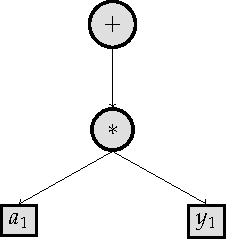
\includegraphics[width=0.3\textwidth]{"figures/mutation_add_term_1.pdf"}
                  \qquad
                  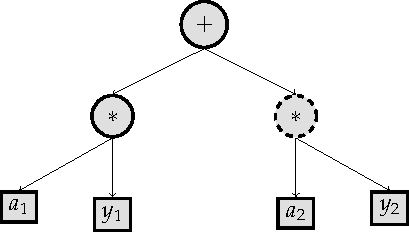
\includegraphics[width=0.5\textwidth]{"figures/mutation_add_term_2.pdf"}
                  \caption{Ejemplo de mutación mediante la adición de un término a una ecuación.}
                  \label{tikzpicture:mutation_add_term}
              \end{figure}
          \end{center}

    \item Mutar un término de la ecuación. Si se toman los sumandos de la ecuación como una lista de términos, el criterio consiste en seleccionar un término y dentro de su representación en forma de árbol computacional, tomar un nodo y aplicarle una de las siguientes modificaciones.
          Si el nodo representa una operación:

          \begin{itemize}
              \item Se cambia la operación en el nodo por uno que posea la misma cantidad de argumentos del operador:

                    Por ejempo, si se tiene el término $y_1 + (y_2 - y_3)$ se puede sustituir la resta por una suma resultando $y_1 + (y_2 + y_3)$. Se muestra en forma de árbol computacional en la figura \ref{tikzpicture:mutation_change_operation}.

                    \begin{center}
                        %   \begin{adjustbox}{width=0.25\textwidth, keepaspectratio}
                        %       \begin{tikzpicture}[
                        %               roundnode_dashed/.style={circle, draw, dashed, fill=gray!25, very thick, minimum size=7mm},
                        %               roundnode/.style={circle, draw, fill=gray!25, very thick, minimum size=7mm},
                        %               squarednode/.style={rectangle, draw, fill=gray!25, very thick, minimum size=5mm},
                        %           ]
                        %           %               %Nodes
                        %           \node[roundnode]      (plus)                            {$+$};
                        %           \node[squarednode]    (y_1)     [below left=of plus]    {$y_1$};
                        %           \node[roundnode_dashed]      (sub)     [below right=of plus]   {$-$};
                        %           \node[squarednode]    (y_2)     [below left=of sub]     {$y_2$};
                        %           \node[squarednode]    (y_3)     [below right=of sub]    {$y_3$};


                        %           %   %Lines
                        %           \draw[->] (plus.south) -- (y_1.north);
                        %           \draw[->] (plus.south) -- (sub.north);
                        %           \draw[->] (sub.south) -- (y_2.north);
                        %           \draw[->] (sub.south) -- (y_3.north);
                        %       \end{tikzpicture}%
                        %   \end{adjustbox}
                        %   \qquad
                        %   \begin{adjustbox}{width=0.25\textwidth, keepaspectratio}
                        %       \begin{tikzpicture}[
                        %               roundnode_dashed/.style={circle, draw, dashed, fill=gray!25, very thick, minimum size=7mm},
                        %               roundnode/.style={circle, draw, fill=gray!25, very thick, minimum size=7mm},
                        %               squarednode/.style={rectangle, draw, fill=gray!25, very thick, minimum size=5mm},
                        %           ]
                        %           %Nodes
                        %           \node[roundnode]      (plus)                            {$+$};
                        %           \node[squarednode]    (y_1)     [below left=of plus]    {$y_1$};
                        %           \node[roundnode_dashed]      (plus_2)     [below right=of plus]   {$+$};
                        %           \node[squarednode]    (y_2)     [below left=of plus_2]     {$y_2$};
                        %           \node[squarednode]    (y_3)     [below right=of plus_2]    {$y_3$};


                        %           %   %Lines
                        %           \draw[->] (plus.south) -- (y_1.north);
                        %           \draw[->] (plus.south) -- (plus_2.north);
                        %           \draw[->] (plus_2.south) -- (y_2.north);
                        %           \draw[->] (plus_2.south) -- (y_3.north);
                        %       \end{tikzpicture}%
                        %   \end{adjustbox}
                        \begin{figure}[h]
                            \centering
                            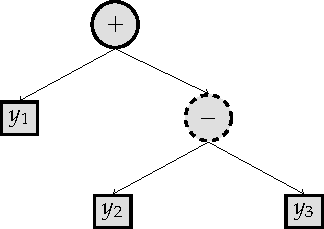
\includegraphics[width=0.3\textwidth]{"figures/mutation_change_operation_1.pdf"}
                            \qquad
                            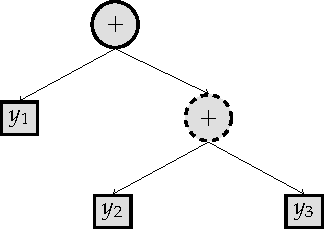
\includegraphics[width=0.3\textwidth]{"figures/mutation_change_operation_2.pdf"}
                            \caption{Ejemplo de mutación mediante la modificación de una operación en un término.}
                            \label{tikzpicture:mutation_change_operation}
                        \end{figure}
                    \end{center}

              \item Se elimina el nodo, colocando en su lugar su primer hijo.

                    Por ejempo, si se tiene el término $y_1 + (y_2 - y_3)$ se puede sustituir la resta por su primer argumento obteniéndose $y_1 + y_2$. Se muestra en forma de árbol computacional en la figura \ref{tikzpicture:mutation_delete_operation}.

                    \begin{center}
                        %   \begin{adjustbox}{width=0.25\textwidth, keepaspectratio}
                        %       \begin{tikzpicture}[
                        %               roundnode_dashed/.style={circle, draw, dashed, fill=gray!25, very thick, minimum size=7mm},
                        %               roundnode/.style={circle, draw, fill=gray!25, very thick, minimum size=7mm},
                        %               squarednode/.style={rectangle, draw, fill=gray!25, very thick, minimum size=5mm},
                        %           ]
                        %           %Nodes
                        %           \node[roundnode]      (plus)                            {$+$};
                        %           \node[squarednode]    (y_1)     [below left=of plus]    {$y_1$};
                        %           \node[roundnode_dashed]      (sub)     [below right=of plus]   {$-$};
                        %           \node[squarednode]    (y_2)     [below left=of sub]     {$y_2$};
                        %           \node[squarednode]    (y_3)     [below right=of sub]    {$y_3$};


                        %           %   %Lines
                        %           \draw[->] (plus.south) -- (y_1.north);
                        %           \draw[->] (plus.south) -- (sub.north);
                        %           \draw[->] (sub.south) -- (y_2.north);
                        %           \draw[->] (sub.south) -- (y_3.north);
                        %       \end{tikzpicture}%
                        %   \end{adjustbox}
                        %   \qquad
                        %   \begin{adjustbox}{width=0.25\textwidth, keepaspectratio}
                        %       \begin{tikzpicture}[
                        %               roundnode_dashed/.style={circle, draw, dashed, fill=gray!25, very thick, minimum size=7mm},
                        %               roundnode/.style={circle, draw, fill=gray!25, very thick, minimum size=7mm},
                        %               squarednode/.style={rectangle, draw, fill=gray!25, very thick, minimum size=5mm},
                        %           ]
                        %           %Nodes
                        %           \node[roundnode]      (plus)                            {$+$};
                        %           \node[squarednode]    (y_1)     [below left=of plus]    {$y_1$};
                        %           \node[squarednode]    (y_2)     [below right=of plus]     {$y_2$};


                        %           %   %Lines
                        %           \draw[->] (plus.south) -- (y_1.north);
                        %           \draw[->] (plus.south) -- (y_2.north);
                        %       \end{tikzpicture}%
                        %   \end{adjustbox}
                        \begin{figure}[h]
                            \centering
                            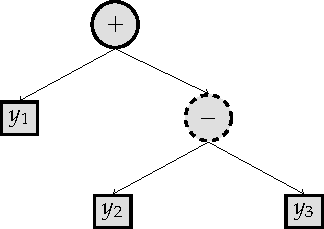
\includegraphics[width=0.3\textwidth]{"figures/mutation_delete_operation_1.pdf"}
                            \qquad
                            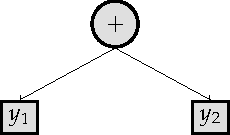
\includegraphics[width=0.3\textwidth]{"figures/mutation_delete_operation_2.pdf"}
                            \caption{Ejemplo de mutación mediante la eliminación de una operación en un término.}
                            \label{tikzpicture:mutation_delete_operation}
                        \end{figure}
                    \end{center}

              \item Se cambia el nodo por uno nuevo que represente una operación aleatoria colocando como hijos nuevos árboles de expresiones aleatorias y como último hijo el nodo original que se seleccionó.

                    Por ejempo, si se tiene el término $y_1 + (y_2 - y_3)$ se puede sustituir la resta por una multiplicación colocando como segundo factor la misma resta obteniéndose $y_1 + y_4 * (y_2 - y_3)$. Se expresa en forma de árbol computacional en la figura \ref{tikzpicture:mutation_add_operation}.

                    \begin{center}
                        %   \begin{adjustbox}{width=0.25\textwidth, keepaspectratio}
                        %       \begin{tikzpicture}[
                        %               roundnode_dashed/.style={circle, draw, dashed, fill=gray!25, very thick, minimum size=7mm},
                        %               roundnode/.style={circle, draw, fill=gray!25, very thick, minimum size=7mm},
                        %               squarednode/.style={rectangle, draw, fill=gray!25, very thick, minimum size=5mm},
                        %           ]
                        %           %Nodes
                        %           \node[roundnode]      (plus)                            {$+$};
                        %           \node[squarednode]    (y_1)     [below left=of plus]    {$y_1$};
                        %           \node[roundnode_dashed]      (sub)     [below right=of plus]   {$-$};
                        %           \node[squarednode]    (y_2)     [below left=of sub]     {$y_2$};
                        %           \node[squarednode]    (y_3)     [below right=of sub]    {$y_3$};


                        %           %   %Lines
                        %           \draw[->] (plus.south) -- (y_1.north);
                        %           \draw[->] (plus.south) -- (sub.north);
                        %           \draw[->] (sub.south) -- (y_2.north);
                        %           \draw[->] (sub.south) -- (y_3.north);
                        %       \end{tikzpicture}%
                        %   \end{adjustbox}
                        %   \qquad
                        %   \begin{adjustbox}{width=0.25\textwidth, keepaspectratio}
                        %       \begin{tikzpicture}[
                        %               roundnode_dashed/.style={circle, draw, dashed, fill=gray!25, very thick, minimum size=7mm},
                        %               roundnode/.style={circle, draw, fill=gray!25, very thick, minimum size=7mm},
                        %               squarednode/.style={rectangle, draw, fill=gray!25, very thick, minimum size=5mm},
                        %           ]
                        %           %Nodes
                        %           \node[roundnode]      (plus)                            {$+$};
                        %           \node[squarednode]    (y_1)     [below left=of plus]    {$y_1$};
                        %           \node[roundnode]    (star)  [below right=of plus]   {$*$};
                        %           \node[squarednode]  (y_4)   [below left=of star]        {$y_4$};
                        %           \node[roundnode_dashed]      (sub)     [below right=of star]   {$-$};
                        %           \node[squarednode]    (y_2)     [below left=of sub]     {$y_2$};
                        %           \node[squarednode]    (y_3)     [below right=of sub]    {$y_3$};


                        %           %   %Lines
                        %           \draw[->] (plus.south) -- (y_1.north);
                        %           \draw[->] (plus.south) -- (star.north);
                        %           \draw[->] (star.south) -- (y_4.north);
                        %           \draw[->] (star.south) -- (sub.north);
                        %           \draw[->] (sub.south) -- (y_2.north);
                        %           \draw[->] (sub.south) -- (y_3.north);
                        %       \end{tikzpicture}%
                        %   \end{adjustbox}
                        \begin{figure}[h]
                            \centering
                            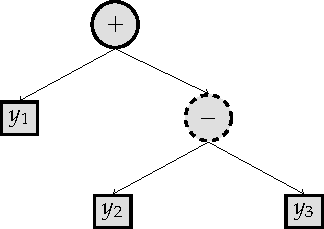
\includegraphics[width=0.4\textwidth]{"figures/mutation_add_operation_1.pdf"}
                            \qquad
                            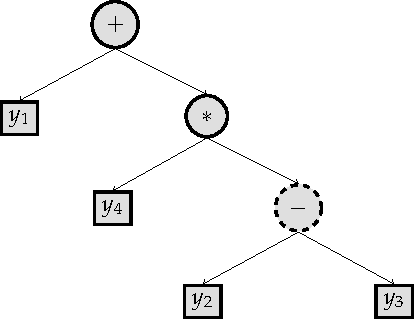
\includegraphics[width=0.4\textwidth]{"figures/mutation_add_operation_2.pdf"}
                            \caption{Ejemplo de mutación mediante la adición de un nuevo nodo a un término.}
                            \label{tikzpicture:mutation_add_operation}
                        \end{figure}
                    \end{center}

          \end{itemize}

          Si el nodo representa una variable:

          \begin{itemize}
              \item Cambiar la variable por otra permitida dentro de la ecuación.

                    Por ejempo, si se tiene el término $y_1 + (y_2 - y_3)$ se puede sustituir la variable $y_3$ obteniéndose $y_1 + (y_2 - y_1)$. Se plantea en forma de árbol computacional en la figura \ref{tikzpicture:mutation_change_variable}.

                    \begin{center}
                        %   \begin{adjustbox}{width=0.25\textwidth, keepaspectratio}
                        %       \begin{tikzpicture}[
                        %               roundnode/.style={circle, draw, fill=gray!25, very thick, minimum size=7mm},
                        %               squarednode/.style={rectangle, draw, fill=gray!25, very thick, minimum size=5mm},
                        %               squarednode_dashed/.style={rectangle, draw, dashed, fill=gray!25, very thick, minimum size=7mm},
                        %           ]
                        %           %Nodes
                        %           \node[roundnode]      (plus)                            {$+$};
                        %           \node[squarednode]    (y_1)     [below left=of plus]    {$y_1$};
                        %           \node[roundnode]      (sub)     [below right=of plus]   {$-$};
                        %           \node[squarednode]    (y_2)     [below left=of sub]     {$y_2$};
                        %           \node[squarednode_dashed]    (y_3)     [below right=of sub]    {$y_3$};


                        %           %   %Lines
                        %           \draw[->] (plus.south) -- (y_1.north);
                        %           \draw[->] (plus.south) -- (sub.north);
                        %           \draw[->] (sub.south) -- (y_2.north);
                        %           \draw[->] (sub.south) -- (y_3.north);
                        %       \end{tikzpicture}%
                        %   \end{adjustbox}
                        %   \qquad
                        %   \begin{adjustbox}{width=0.25\textwidth, keepaspectratio}
                        %       \begin{tikzpicture}[
                        %               roundnode/.style={circle, draw, fill=gray!25, very thick, minimum size=7mm},
                        %               squarednode/.style={rectangle, draw, fill=gray!25, very thick, minimum size=5mm},
                        %               squarednode_dashed/.style={rectangle, draw, dashed, fill=gray!25, very thick, minimum size=7mm},
                        %           ]
                        %           %Nodes
                        %           \node[roundnode]      (plus)                            {$+$};
                        %           \node[squarednode]    (y_1)     [below left=of plus]    {$y_1$};
                        %           \node[roundnode]      (sub)     [below right=of plus]   {$-$};
                        %           \node[squarednode]    (y_2)     [below left=of sub]     {$y_2$};
                        %           \node[squarednode_dashed]    (y_1_2)     [below right=of sub]    {$y_1$};


                        %           %   %Lines
                        %           \draw[->] (plus.south) -- (y_1.north);
                        %           \draw[->] (plus.south) -- (sub.north);
                        %           \draw[->] (sub.south) -- (y_2.north);
                        %           \draw[->] (sub.south) -- (y_1_2.north);
                        %       \end{tikzpicture}%
                        %   \end{adjustbox}
                        \begin{figure}[!h]
                            \centering
                            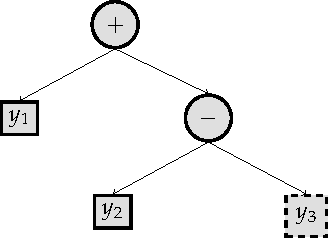
\includegraphics[width=0.3\textwidth]{"figures/mutation_change_variable_1.pdf"}
                            \qquad
                            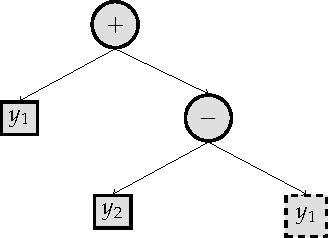
\includegraphics[width=0.3\textwidth]{"figures/mutation_change_variable_2.pdf"}
                            \caption{Ejemplo de mutación mediante la modificación de una variable un término.}
                            \label{tikzpicture:mutation_change_variable}
                        \end{figure}
                    \end{center}

              \item Cambiar la variable por un nodo que represente una operación aleatoria donde el primer hijo es la variable seleccionada y el resto de hijos son nuevos árboles de expresiones aleatorias.

                    Por ejempo, si se tiene el término $y_1 + (y_2 - y_3)$ se puede sustituir la variable $y_3$ por una multiplicación donde el primer factor sea la misma variable $y_3$ y el segundo factor sea la variable $y_2$, obteniéndose $y_1 + (y_2 - y_3 * y_2)$. Se expresa en forma de árbol computacional en la figura \ref{tikzpicture:mutation_change_variable_by_node}.

                    \begin{center}
                        %   \begin{adjustbox}{width=0.25\textwidth, keepaspectratio}
                        %       \begin{tikzpicture}[
                        %               roundnode/.style={circle, draw, fill=gray!25, very thick, minimum size=7mm},
                        %               squarednode/.style={rectangle, draw, fill=gray!25, very thick, minimum size=5mm},
                        %               squarednode_dashed/.style={rectangle, draw, dashed, fill=gray!25, very thick, minimum size=7mm},
                        %           ]
                        %           %Nodes
                        %           \node[roundnode]      (plus)                            {$+$};
                        %           \node[squarednode]    (y_1)     [below left=of plus]    {$y_1$};
                        %           \node[roundnode]      (sub)     [below right=of plus]   {$-$};
                        %           \node[squarednode]    (y_2)     [below left=of sub]     {$y_2$};
                        %           \node[squarednode_dashed]    (y_3)     [below right=of sub]    {$y_3$};


                        %           %   %Lines
                        %           \draw[->] (plus.south) -- (y_1.north);
                        %           \draw[->] (plus.south) -- (sub.north);
                        %           \draw[->] (sub.south) -- (y_2.north);
                        %           \draw[->] (sub.south) -- (y_3.north);
                        %       \end{tikzpicture}%
                        %   \end{adjustbox}
                        %   \qquad
                        %   \begin{adjustbox}{width=0.25\textwidth, keepaspectratio}
                        %       \begin{tikzpicture}[
                        %               roundnode/.style={circle, draw, fill=gray!25, very thick, minimum size=7mm},
                        %               squarednode/.style={rectangle, draw, fill=gray!25, very thick, minimum size=5mm},
                        %               squarednode_dashed/.style={rectangle, draw, dashed, fill=gray!25, very thick, minimum size=7mm},
                        %           ]
                        %           %Nodes
                        %           \node[roundnode]      (plus)                            {$+$};
                        %           \node[squarednode]    (y_1)     [below left=of plus]    {$y_1$};
                        %           \node[roundnode]    (sub)  [below right=of plus]   {$-$};
                        %           \node[squarednode]  (y_2)   [below left=of sub]        {$y_2$};
                        %           \node[roundnode]      (star)     [below right=of sub]   {$*$};
                        %           \node[squarednode_dashed]    (y_3)     [below left=of star]    {$y_3$};
                        %           \node[squarednode]    (y_2_2)     [below right=of star]     {$y_2$};


                        %           %   %Lines
                        %           \draw[->] (plus.south) -- (y_1.north);
                        %           \draw[->] (plus.south) -- (sub.north);
                        %           \draw[->] (sub.south) -- (y_2.north);
                        %           \draw[->] (sub.south) -- (star.north);
                        %           \draw[->] (star.south) -- (y_3.north);
                        %           \draw[->] (star.south) -- (y_2_2.north);
                        %       \end{tikzpicture}%
                        %   \end{adjustbox}
                        \begin{figure}[h]
                            \centering
                            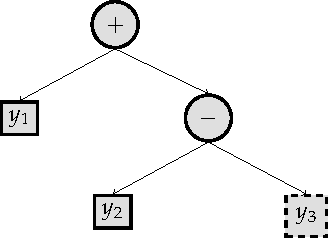
\includegraphics[width=0.4\textwidth]{"figures/mutation_change_variable_by_node_1.pdf"}
                            \qquad
                            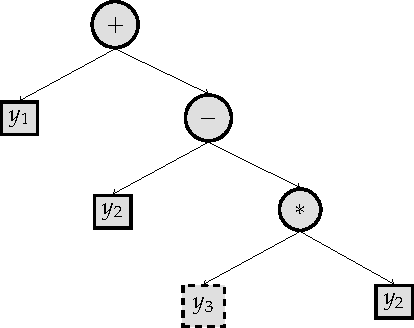
\includegraphics[width=0.4\textwidth]{"figures/mutation_change_variable_by_node_2.pdf"}
                            \caption{Ejemplo de mutación mediante la modificación de un nodo representante de una variable por una operación en un término.}
                            \label{tikzpicture:mutation_change_variable_by_node}
                        \end{figure}
                    \end{center}
          \end{itemize}
\end{itemize}

Como ejemplo de una operación de mutación se puede tomar el sistema:
\begin{align*}
    S' & = - a_1 * S * I         \\
    I' & = a_2 * S * I - a_3 * I \\
    R' & = a_4 * I,
\end{align*}
y se puede realizar la mutación de eliminar el segundo término de la segunda ecuación quedando como resultado el sistema:
\begin{align*}
    S' & = - a_1 * S * I \\
    I' & = a_2 * S * I   \\
    R' & = a_4 * I,
\end{align*}

Este ejemplo se representa en forma de árbol computacional en la figura \ref{tikzpicture:mutation_sir} de la página \pageref{tikzpicture:mutation_sir}.

\begin{center}
    % \begin{adjustbox}{width=0.5\textwidth, keepaspectratio}
    %     \begin{tikzpicture}[
    %             roundnode/.style={circle, draw, fill=gray!25, very thick, minimum size=7mm},
    %             squarednode/.style={rectangle, draw, fill=gray!25, very thick, minimum size=5mm},
    %             roundnode_dashed/.style={circle, draw, dashed, fill=gray!25, very thick, minimum size=7mm},
    %         ]
    %         % Nodes
    %         \node[roundnode]        (system)                            {$SYSTEM$};

    %         \node[roundnode]        (plus_S)     [below left=of system]        {$+$};
    %         \node[roundnode]        (star_S_1)    [below left=of plus_S]    {$*$};
    %         \node[squarednode]      (alpha_star_S_1)      [below left=of star_S_1]    {$a_1$};
    %         \node[roundnode]        (neg_star_S_1)    [below=of star_S_1]    {$-$};
    %         \node[roundnode]        (star_S_2)    [below=of neg_star_S_1]    {$*$};
    %         \node[squarednode]      (S_star_S)       [below left=of star_S_2]   {$S$};
    %         \node[squarednode]      (I_star_S)      [below=of star_S_2]   {$I$};

    %         \node[roundnode]        (plus_I)     [below=of system]        {$+$};
    %         \node[roundnode]        (star_I_1)    [below left=of plus_I]    {$*$};
    %         \node[squarednode]      (alpha_star_I_1)      [below left=1cm and 0.5cm of star_I_1]    {$a_2$};
    %         \node[roundnode]        (star_I_2)    [below=of star_I_1]    {$*$};
    %         \node[squarednode]      (S_star_I)       [below left=1cm and 0.5cm of star_I_2]   {$S$};
    %         \node[squarednode]      (I_star_I_1)      [below=of star_I_2]   {$I$};

    %         \node[roundnode_dashed]        (star_I_3)    [below right=of plus_I]    {$*$};
    %         \node[squarednode]      (beta_star_I_1)      [below=of star_I_3]    {$a_3$};
    %         \node[roundnode]        (neg_star_I_1)    [below right=1cm and 0.5cm of star_I_3]    {$-$};
    %         \node[squarednode]      (I_star_I_2)      [below=of neg_star_I_1]   {$I$};

    %         \node[roundnode]        (plus_R)     [below right=of system]        {$+$};
    %         \node[roundnode]        (star_R_1)    [below right=of plus_R]    {$*$};
    %         \node[squarednode]      (beta_star_R_1)      [below=of star_R_1]    {$a_4$};
    %         \node[squarednode]      (I_star_R)      [below right=of star_R_1]   {$I$};

    %         %Lines
    %         \draw [->] (system.south) -- (plus_S.north);
    %         \draw[->] (system.south) -- (plus_I.north);
    %         \draw[->] (system.south) -- (plus_R.north);

    %         \draw[->] (plus_S.south) -- (star_S_1.north);
    %         \draw[->] (star_S_1.south) -- (alpha_star_S_1.north);
    %         \draw[->] (star_S_1.south) -- (neg_star_S_1.north);
    %         \draw[->] (neg_star_S_1.south) -- (star_S_2.north);
    %         \draw[->] (star_S_2.south) -- (S_star_S.north);
    %         \draw[->] (star_S_2.south) -- (I_star_S.north);

    %         \draw[->] (plus_I.south) -- (star_I_1.north);
    %         \draw[->] (plus_I.south) -- (star_I_3.north);
    %         \draw[->] (star_I_1.south) -- (alpha_star_I_1.north);
    %         \draw[->] (star_I_1.south) -- (star_I_2.north);
    %         \draw[->] (star_I_2.south) -- (S_star_I.north);
    %         \draw[->] (star_I_2.south) -- (I_star_I_1.north);

    %         \draw[->] (star_I_3.south) -- (beta_star_I_1.north);
    %         \draw[->] (star_I_3.south) -- (neg_star_I_1.north);
    %         \draw[->] (neg_star_I_1.south) -- (I_star_I_2.north);

    %         \draw[->] (plus_R.south) -- (star_R_1.north);
    %         \draw[->] (star_R_1.south) -- (beta_star_R_1.north);
    %         \draw[->] (star_R_1.south) -- (I_star_R.north);
    %     \end{tikzpicture}
    % \end{adjustbox}

    \begin{figure}[h]
        \centering
        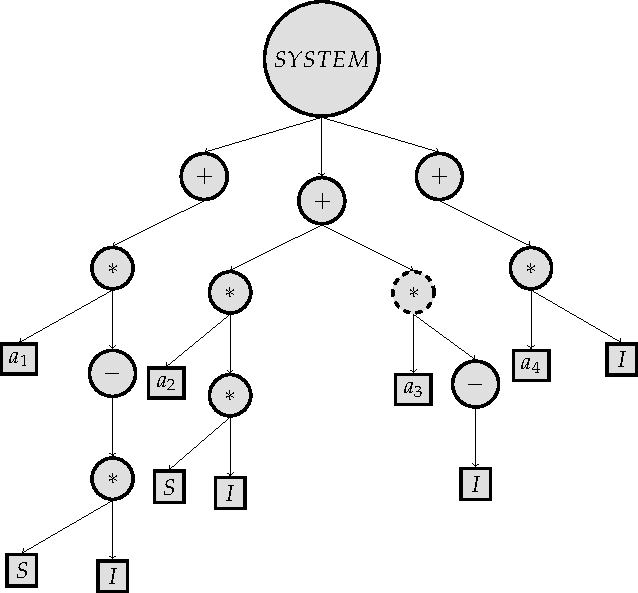
\includegraphics[width=0.6\textwidth]{"figures/mutation_sir_1.pdf"}
        \qquad
        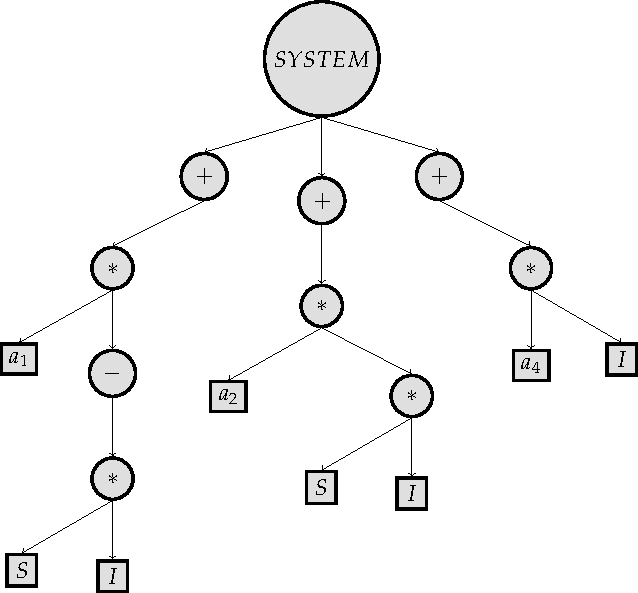
\includegraphics[width=0.6\textwidth]{"figures/mutation_sir_2.pdf"}
        \caption{Ejemplo de mutación mediante la eliminación de un término en una ecuación.}
        \label{tikzpicture:mutation_sir}
    \end{figure}

\end{center}

% \begin{center}
%     \begin{adjustbox}{width=0.5\textwidth, keepaspectratio}
%         \begin{tikzpicture}[
%                 roundnode/.style={circle, draw, fill=gray!25, very thick, minimum size=7mm},
%                 squarednode/.style={rectangle, draw, fill=gray!25, very thick, minimum size=5mm},
%                 roundnode_dashed/.style={circle, draw, dashed, fill=gray!25, very thick, minimum size=7mm},
%             ]
%             % Nodes
%             \node[roundnode]        (system)                            {$SYSTEM$};

%             \node[roundnode]        (plus_S)     [below left=of system]        {$+$};
%             \node[roundnode]        (star_S_1)    [below left=of plus_S]    {$*$};
%             \node[squarednode]      (alpha_star_S_1)      [below left=of star_S_1]    {$a_1$};
%             \node[roundnode]        (neg_star_S_1)    [below=of star_S_1]    {$-$};
%             \node[roundnode]        (star_S_2)    [below=of neg_star_S_1]    {$*$};
%             \node[squarednode]      (S_star_S)       [below left=of star_S_2]   {$S$};
%             \node[squarednode]      (I_star_S)      [below=of star_S_2]   {$I$};

%             \node[roundnode]        (plus_I)     [below=of system]        {$+$};
%             \node[roundnode]        (star_I_1)    [below=of plus_I]    {$*$};
%             \node[squarednode]      (alpha_star_I_1)      [below left=of star_I_1]    {$a_2$};
%             \node[roundnode]        (star_I_2)    [below right=of star_I_1]    {$*$};
%             \node[squarednode]      (S_star_I)       [below left=of star_I_2]   {$S$};
%             \node[squarednode]      (I_star_I_1)      [below=of star_I_2]   {$I$};

%             \node[roundnode]        (plus_R)     [below right=of system]        {$+$};
%             \node[roundnode]        (star_R_1)    [below right=of plus_R]    {$*$};
%             \node[squarednode]      (beta_star_R_1)      [below=of star_R_1]    {$a_4$};
%             \node[squarednode]      (I_star_R)      [below right=of star_R_1]   {$I$};

%             %Lines
%             \draw [->] (system.south) -- (plus_S.north);
%             \draw[->] (system.south) -- (plus_I.north);
%             \draw[->] (system.south) -- (plus_R.north);

%             \draw[->] (plus_S.south) -- (star_S_1.north);
%             \draw[->] (star_S_1.south) -- (alpha_star_S_1.north);
%             \draw[->] (star_S_1.south) -- (neg_star_S_1.north);
%             \draw[->] (neg_star_S_1.south) -- (star_S_2.north);
%             \draw[->] (star_S_2.south) -- (S_star_S.north);
%             \draw[->] (star_S_2.south) -- (I_star_S.north);

%             \draw[->] (plus_I.south) -- (star_I_1.north);
%             \draw[->] (star_I_1.south) -- (alpha_star_I_1.north);
%             \draw[->] (star_I_1.south) -- (star_I_2.north);
%             \draw[->] (star_I_2.south) -- (S_star_I.north);
%             \draw[->] (star_I_2.south) -- (I_star_I_1.north);

%             \draw[->] (plus_R.south) -- (star_R_1.north);
%             \draw[->] (star_R_1.south) -- (beta_star_R_1.north);
%             \draw[->] (star_R_1.south) -- (I_star_R.north);
%         \end{tikzpicture}
%     \end{adjustbox}
% \end{center}

Con estas modificaciones que se le pueden realizar a un sistema de ecuaciones diferenciales lineales con respecto a los parámetros se define la operación de mutación que se utiliza en el algoritmo genético que se emplea en este trabajo. Otra de las operaciones que se deben definir con el fin de implementar un algoritmo genético es el cruzamiento, que se describe en la siguiente sección.

\section{Cruzamiento}\label{section:xcross}

En la operación de cruzamiento se obtiene un nuevo sistema de ecuaciones diferenciales combinando propiedades de dos sistemas existentes A y B. Esta operación selecciona un nodo aleatorio dentro del árbol A que no represente un parámetro y un nodo dentro del árbol B que tampoco represente un parámetro, siguiendo un conjunto de reglas. Una vez escogidos los nodos se remplaza el subárbol del nodo seleccionado en A por el subárbol del nodo seleccionado en B, resultando en A un nuevo sistema de ecuaciones diferenciales.

En dependencia del nodo seleccionado en A se escoge el nodo en B siguiendo las siguientes reglas:


\begin{itemize}
    \item Si el nodo seleccionado en A es el representante de la i-ésima ecuación en el sistema, se escoge el nodo representante de la i-ésima ecuación en el sistema B. Se puede ver como ejemplo la figura \ref{tikzpicture:cross_equation} de la página \pageref{tikzpicture:cross_equation}.

          \begin{center}
              %   \begin{adjustbox}{width=0.4\textwidth, keepaspectratio}
              %       \begin{tikzpicture}[
              %               roundnode/.style={circle, draw, fill=gray!25, very thick, minimum size=7mm},
              %               squarednode/.style={rectangle, draw, fill=gray!25, very thick, minimum size=5mm},
              %               roundnode_dashed/.style={circle, draw, dashed, fill=gray!25, very thick, minimum size=7mm},
              %           ]
              %           % Nodes
              %           \node[roundnode]        (system)                            {$A$};

              %           \node[roundnode]        (plus_1)     [below left=of system]        {$+$};
              %           \node[roundnode]        (star_1_1)    [below=of plus_1]    {$*$};
              %           \node[squarednode]      (a_1)      [below left=of star_1_1]    {$a_1$};
              %           \node[roundnode]        (star_1_2)    [below=of star_1_1]    {$*$};
              %           \node[squarednode]      (S_star_1_2)       [below left=of star_1_2]   {$y_1$};
              %           \node[squarednode]      (I_star_1_2)      [below=of star_1_2]   {$y_2$};

              %           \node[roundnode_dashed]        (plus_2)     [below right=of system]        {$+$};
              %           \node[roundnode]        (star_2_1)    [below=of plus_2]    {$*$};
              %           \node[squarednode]      (a_2)      [below=of star_2_1]    {$a_2$};
              %           \node[squarednode]      (I_star_2_1)      [below right=of star_2_1]   {$y_2$};

              %           %Lines
              %           \draw [->] (system.south) -- (plus_1.north);
              %           \draw[->] (system.south) -- (plus_2.north);
              %           \draw[->] (plus_1.south) -- (star_1_1.north);
              %           \draw[->] (plus_2.south) -- (star_2_1.north);
              %           \draw[->] (star_1_1.south) -- (a_1.north);
              %           \draw[->] (star_1_1.south) -- (star_1_2.north);
              %           \draw[->] (star_1_2.south) -- (S_star_1_2.north);
              %           \draw[->] (star_1_2.south) -- (I_star_1_2.north);
              %           \draw[->] (star_2_1.south) -- (a_2.north);
              %           \draw[->] (star_2_1.south) -- (I_star_2_1.north);
              %       \end{tikzpicture}
              %   \end{adjustbox}
              %   \qquad
              %   \begin{adjustbox}{width=0.4\textwidth, keepaspectratio}
              %       \begin{tikzpicture}[
              %               roundnode/.style={circle, draw, fill=gray!25, very thick, minimum size=7mm},
              %               squarednode/.style={rectangle, draw, fill=gray!25, very thick, minimum size=5mm},
              %               roundnode_dashed/.style={circle, draw, dashed, fill=gray!25, very thick, minimum size=7mm},
              %           ]
              %           % Nodes
              %           \node[roundnode]        (system)                            {$B$};

              %           \node[roundnode]        (plus_1)     [below left=of system]        {$+$};
              %           \node[roundnode]        (star_1_1)    [below=of plus_1]    {$*$};
              %           \node[squarednode]      (a_3)      [below left=of star_1_1]    {$b_1$};
              %           \node[roundnode]        (plus_1_2)    [below=of star_1_1]    {$+$};
              %           \node[squarednode]      (I_plus_1_2)       [below left=of plus_1_2]   {$y_2$};
              %           \node[squarednode]      (S_plus_1_2)      [below=of plus_1_2]   {$y_1$};

              %           \node[roundnode_dashed]        (plus_2)     [below right=of system]        {$+$};
              %           \node[roundnode]        (star_2_1)    [below=of plus_2]    {$*$};
              %           \node[squarednode]      (a_4)      [below=of star_2_1]    {$b_2$};
              %           \node[roundnode]        (sub_2_1)    [below right=of star_2_1]    {$-$};
              %           \node[squarednode]      (S_sub_2_1)       [below left=of sub_2_1]   {$y_1$};
              %           \node[squarednode]      (I_sub_2_1)      [below=of sub_2_1]   {$y_2$};

              %           %Lines
              %           \draw [->] (system.south) -- (plus_1.north);
              %           \draw[->] (system.south) -- (plus_2.north);
              %           \draw[->] (plus_1.south) -- (star_1_1.north);
              %           \draw[->] (plus_2.south) -- (star_2_1.north);
              %           \draw[->] (star_1_1.south) -- (a_3.north);
              %           \draw[->] (star_1_1.south) -- (plus_1_2.north);
              %           \draw[->] (plus_1_2.south) -- (I_plus_1_2.north);
              %           \draw[->] (plus_1_2.south) -- (S_plus_1_2.north);
              %           \draw[->] (star_2_1.south) -- (a_4.north);
              %           \draw[->] (star_2_1.south) -- (sub_2_1.north);
              %           \draw[->] (sub_2_1.south) -- (S_sub_2_1.north);
              %           \draw[->] (sub_2_1.south) -- (I_sub_2_1.north);
              %       \end{tikzpicture}
              %   \end{adjustbox}
              \begin{figure}[h]
                  \centering
                  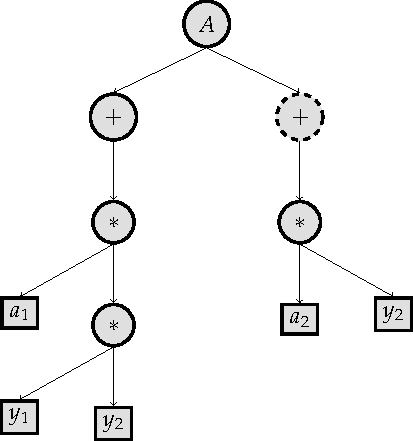
\includegraphics[width=0.4\textwidth]{"figures/cross_equation_1.pdf"}
                  \qquad
                  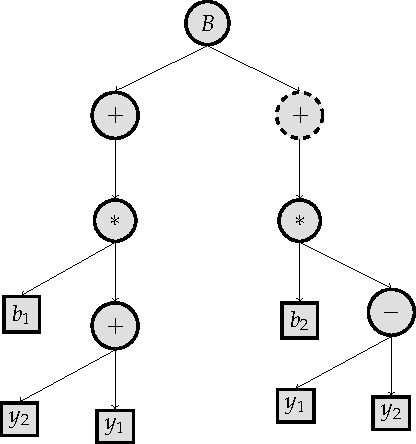
\includegraphics[width=0.4\textwidth]{"figures/cross_equation_2.pdf"}
                  \caption{Ejemplo de selección de un nodo en B cuando en A se selecciona el nodo representante de una ecuación.}
                  \label{tikzpicture:cross_equation}
              \end{figure}
          \end{center}

    \item Si se selecciona en A un nodo representante de un término en la ecuación i-ésima, se escoge un nodo representante de un término en la i-ésima ecuación en el sistema B. Se puede ver como ejemplo la figura \ref{tikzpicture:cross_term} de la página \pageref{tikzpicture:cross_term}.

          \begin{center}
              %   \begin{adjustbox}{width=0.4\textwidth, keepaspectratio}
              %       \begin{tikzpicture}[
              %               roundnode/.style={circle, draw, fill=gray!25, very thick, minimum size=7mm},
              %               squarednode/.style={rectangle, draw, fill=gray!25, very thick, minimum size=5mm},
              %               roundnode_dashed/.style={circle, draw, dashed, fill=gray!25, very thick, minimum size=7mm},
              %           ]
              %           % Nodes
              %           \node[roundnode]        (system)                            {$A$};

              %           \node[roundnode]        (plus_1)     [below left=of system]        {$+$};
              %           \node[roundnode_dashed]        (star_1_1)    [below=of plus_1]    {$*$};
              %           \node[squarednode]      (a_1)      [below left=of star_1_1]    {$a_1$};
              %           \node[roundnode]        (star_1_2)    [below=of star_1_1]    {$*$};
              %           \node[squarednode]      (S_star_1_2)       [below left=of star_1_2]   {$y_1$};
              %           \node[squarednode]      (I_star_1_2)      [below=of star_1_2]   {$y_2$};

              %           \node[roundnode]        (plus_2)     [below right=of system]        {$+$};
              %           \node[roundnode]        (star_2_1)    [below=of plus_2]    {$*$};
              %           \node[squarednode]      (a_2)      [below=of star_2_1]    {$a_2$};
              %           \node[squarednode]      (I_star_2_1)      [below right=of star_2_1]   {$y_2$};

              %           %Lines
              %           \draw [->] (system.south) -- (plus_1.north);
              %           \draw[->] (system.south) -- (plus_2.north);
              %           \draw[->] (plus_1.south) -- (star_1_1.north);
              %           \draw[->] (plus_2.south) -- (star_2_1.north);
              %           \draw[->] (star_1_1.south) -- (a_1.north);
              %           \draw[->] (star_1_1.south) -- (star_1_2.north);
              %           \draw[->] (star_1_2.south) -- (S_star_1_2.north);
              %           \draw[->] (star_1_2.south) -- (I_star_1_2.north);
              %           \draw[->] (star_2_1.south) -- (a_2.north);
              %           \draw[->] (star_2_1.south) -- (I_star_2_1.north);
              %       \end{tikzpicture}
              %   \end{adjustbox}
              %   \qquad
              %   \begin{adjustbox}{width=0.4\textwidth, keepaspectratio}
              %       \begin{tikzpicture}[
              %               roundnode/.style={circle, draw, fill=gray!25, very thick, minimum size=7mm},
              %               squarednode/.style={rectangle, draw, fill=gray!25, very thick, minimum size=5mm},
              %               roundnode_dashed/.style={circle, draw, dashed, fill=gray!25, very thick, minimum size=7mm},
              %           ]
              %           % Nodes
              %           \node[roundnode]        (system)                            {$B$};

              %           \node[roundnode]        (plus_1)     [below left=of system]        {$+$};
              %           \node[roundnode_dashed]        (star_1_1)    [below=of plus_1]    {$*$};
              %           \node[squarednode]      (a_3)      [below left=of star_1_1]    {$b_1$};
              %           \node[roundnode]        (plus_1_2)    [below=of star_1_1]    {$+$};
              %           \node[squarednode]      (I_plus_1_2)       [below left=of plus_1_2]   {$y_2$};
              %           \node[squarednode]      (S_plus_1_2)      [below=of plus_1_2]   {$y_1$};

              %           \node[roundnode]        (plus_2)     [below right=of system]        {$+$};
              %           \node[roundnode]        (star_2_1)    [below=of plus_2]    {$*$};
              %           \node[squarednode]      (a_4)      [below=of star_2_1]    {$b_2$};
              %           \node[roundnode]        (sub_2_1)    [below right=of star_2_1]    {$-$};
              %           \node[squarednode]      (S_sub_2_1)       [below left=of sub_2_1]   {$y_1$};
              %           \node[squarednode]      (I_sub_2_1)      [below=of sub_2_1]   {$y_2$};

              %           %Lines
              %           \draw [->] (system.south) -- (plus_1.north);
              %           \draw[->] (system.south) -- (plus_2.north);
              %           \draw[->] (plus_1.south) -- (star_1_1.north);
              %           \draw[->] (plus_2.south) -- (star_2_1.north);
              %           \draw[->] (star_1_1.south) -- (a_3.north);
              %           \draw[->] (star_1_1.south) -- (plus_1_2.north);
              %           \draw[->] (plus_1_2.south) -- (I_plus_1_2.north);
              %           \draw[->] (plus_1_2.south) -- (S_plus_1_2.north);
              %           \draw[->] (star_2_1.south) -- (a_4.north);
              %           \draw[->] (star_2_1.south) -- (sub_2_1.north);
              %           \draw[->] (sub_2_1.south) -- (S_sub_2_1.north);
              %           \draw[->] (sub_2_1.south) -- (I_sub_2_1.north);
              %       \end{tikzpicture}
              %   \end{adjustbox}
              \begin{figure}[h]
                  \centering
                  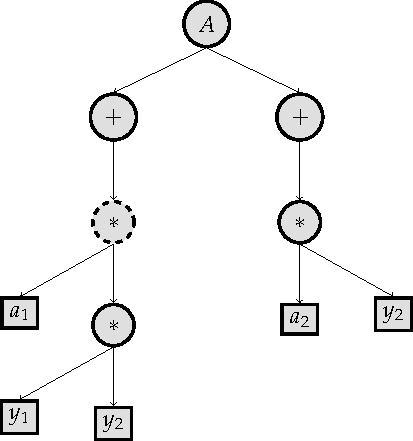
\includegraphics[width=0.4\textwidth]{"figures/cross_term_1.pdf"}
                  \qquad
                  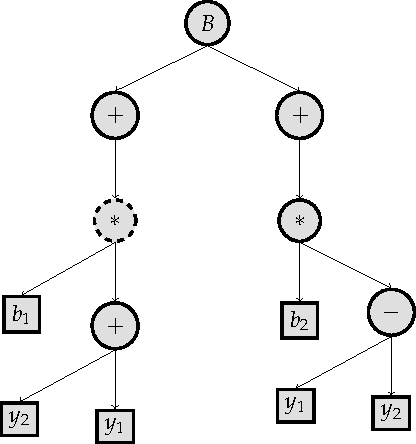
\includegraphics[width=0.4\textwidth]{"figures/cross_term_2.pdf"}
                  \caption{Ejemplo de selección de un nodo en B cuando en A se selecciona el nodo representante de un término en la primera ecuación.}
                  \label{tikzpicture:cross_term}
              \end{figure}
          \end{center}


    \item Si el nodo seleccionado en A es el representante de una operación o una variable perteneciente a la i-ésima ecuación, se selecciona un nodo representante de una operación o una variable que pertenezca a algún término en la i-ésima ecuación en el sistema B. Se puede ver como ejemplo la figura \ref{tikzpicture:cross_operation} de la página \pageref{tikzpicture:cross_operation}.

          \begin{center}
              %   \begin{adjustbox}{width=0.4\textwidth, keepaspectratio}
              %       \begin{tikzpicture}[
              %               roundnode/.style={circle, draw, fill=gray!25, very thick, minimum size=7mm},
              %               squarednode/.style={rectangle, draw, fill=gray!25, very thick, minimum size=5mm},
              %               squarednode_dashed/.style={rectangle, draw, dashed, fill=gray!25, very thick, minimum size=7mm},
              %           ]
              %           % Nodes
              %           \node[roundnode]        (system)                            {$A$};

              %           \node[roundnode]        (plus_1)     [below left=of system]        {$+$};
              %           \node[roundnode]        (star_1_1)    [below=of plus_1]    {$*$};
              %           \node[squarednode]      (a_1)      [below left=of star_1_1]    {$a_1$};
              %           \node[roundnode]        (star_1_2)    [below=of star_1_1]    {$*$};
              %           \node[squarednode]      (S_star_1_2)       [below left=of star_1_2]   {$y_1$};
              %           \node[squarednode]      (I_star_1_2)      [below=of star_1_2]   {$y_2$};

              %           \node[roundnode]        (plus_2)     [below right=of system]        {$+$};
              %           \node[roundnode]        (star_2_1)    [below=of plus_2]    {$*$};
              %           \node[squarednode]      (a_2)      [below=of star_2_1]    {$a_2$};
              %           \node[squarednode_dashed]      (I_star_2_1)      [below right=of star_2_1]   {$y_2$};

              %           %Lines
              %           \draw [->] (system.south) -- (plus_1.north);
              %           \draw[->] (system.south) -- (plus_2.north);
              %           \draw[->] (plus_1.south) -- (star_1_1.north);
              %           \draw[->] (plus_2.south) -- (star_2_1.north);
              %           \draw[->] (star_1_1.south) -- (a_1.north);
              %           \draw[->] (star_1_1.south) -- (star_1_2.north);
              %           \draw[->] (star_1_2.south) -- (S_star_1_2.north);
              %           \draw[->] (star_1_2.south) -- (I_star_1_2.north);
              %           \draw[->] (star_2_1.south) -- (a_2.north);
              %           \draw[->] (star_2_1.south) -- (I_star_2_1.north);
              %       \end{tikzpicture}
              %   \end{adjustbox}
              %   \qquad
              %   \begin{adjustbox}{width=0.4\textwidth, keepaspectratio}
              %       \begin{tikzpicture}[
              %               roundnode/.style={circle, draw, fill=gray!25, very thick, minimum size=7mm},
              %               squarednode/.style={rectangle, draw, fill=gray!25, very thick, minimum size=5mm},
              %               roundnode_dashed/.style={circle, draw, dashed, fill=gray!25, very thick, minimum size=7mm},
              %           ]
              %           % Nodes
              %           \node[roundnode]        (system)                            {$B$};

              %           \node[roundnode]        (plus_1)     [below left=of system]        {$+$};
              %           \node[roundnode]        (star_1_1)    [below=of plus_1]    {$*$};
              %           \node[squarednode]      (a_3)      [below left=of star_1_1]    {$b_1$};
              %           \node[roundnode]        (plus_1_2)    [below=of star_1_1]    {$+$};
              %           \node[squarednode]      (I_plus_1_2)       [below left=of plus_1_2]   {$y_2$};
              %           \node[squarednode]      (S_plus_1_2)      [below=of plus_1_2]   {$y_1$};

              %           \node[roundnode]        (plus_2)     [below right=of system]        {$+$};
              %           \node[roundnode]        (star_2_1)    [below=of plus_2]    {$*$};
              %           \node[squarednode]      (a_4)      [below=of star_2_1]    {$b_2$};
              %           \node[roundnode_dashed]        (sub_2_1)    [below right=of star_2_1]    {$-$};
              %           \node[squarednode]      (S_sub_2_1)       [below left=of sub_2_1]   {$y_1$};
              %           \node[squarednode]      (I_sub_2_1)      [below=of sub_2_1]   {$y_2$};

              %           %Lines
              %           \draw [->] (system.south) -- (plus_1.north);
              %           \draw[->] (system.south) -- (plus_2.north);
              %           \draw[->] (plus_1.south) -- (star_1_1.north);
              %           \draw[->] (plus_2.south) -- (star_2_1.north);
              %           \draw[->] (star_1_1.south) -- (a_3.north);
              %           \draw[->] (star_1_1.south) -- (plus_1_2.north);
              %           \draw[->] (plus_1_2.south) -- (I_plus_1_2.north);
              %           \draw[->] (plus_1_2.south) -- (S_plus_1_2.north);
              %           \draw[->] (star_2_1.south) -- (a_4.north);
              %           \draw[->] (star_2_1.south) -- (sub_2_1.north);
              %           \draw[->] (sub_2_1.south) -- (S_sub_2_1.north);
              %           \draw[->] (sub_2_1.south) -- (I_sub_2_1.north);
              %       \end{tikzpicture}
              %   \end{adjustbox}
              \begin{figure}[H]
                  \centering
                  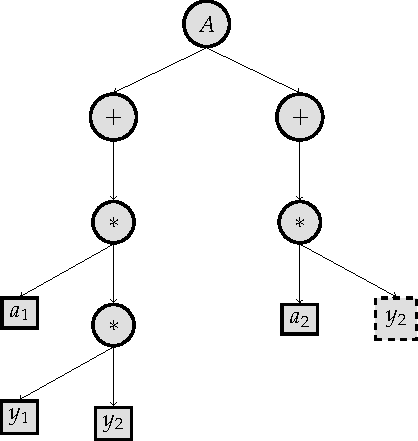
\includegraphics[width=0.37\textwidth]{"figures/cross_operation_1.pdf"}
                  \qquad
                  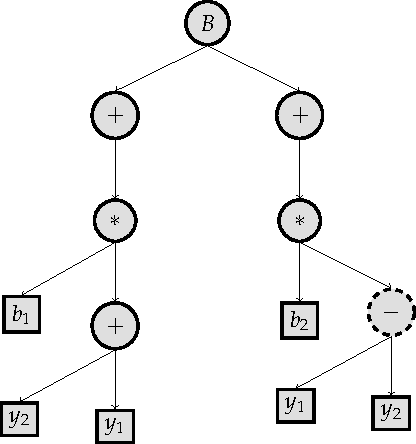
\includegraphics[width=0.37\textwidth]{"figures/cross_operation_2.pdf"}
                  \caption{Ejemplo de selección de un nodo en B cuando en A se selecciona el nodo representante de una variable en la segunda ecuación.}
                  \label{tikzpicture:cross_operation}
              \end{figure}
          \end{center}

\end{itemize}

Por ejemplo, si se tiene el sistema $A$:
\begin{align*}
    S' & = - a_1 * S * I         \\
    I' & = a_2 * S * I - a_3 * I \\
    R' & = a_4 * I,
\end{align*}
y el sistema B:
\begin{align*}
    S' & = b_1 * (S + I) \\
    I' & = b_2 * S * I   \\
    R' & = b_3 * S,
\end{align*}
donde su representación computacional aparece en la figura \ref{tikzpicture:cross_example_1} de la página \pageref{tikzpicture:cross_example_1},
\begin{center}
    % \begin{adjustbox}{width=0.5\textwidth, keepaspectratio}
    %     \begin{tikzpicture}[
    %             roundnode/.style={circle, draw, fill=gray!25, very thick, minimum size=7mm},
    %             squarednode/.style={rectangle, draw, fill=gray!25, very thick, minimum size=5mm},
    %             roundnode_dashed/.style={circle, draw, dashed, fill=gray!25, very thick, minimum size=7mm},
    %         ]
    %         % Nodes
    %         \node[roundnode]        (system)                            {$A$};

    %         \node[roundnode]        (plus_S)     [below left=of system]        {$+$};
    %         \node[roundnode]        (star_S_1)    [below left=of plus_S]    {$*$};
    %         \node[squarednode]      (alpha_star_S_1)      [below left=of star_S_1]    {$a_1$};
    %         \node[roundnode]        (neg_star_S_1)    [below=of star_S_1]    {$-$};
    %         \node[roundnode]        (star_S_2)    [below=of neg_star_S_1]    {$*$};
    %         \node[squarednode]      (S_star_S)       [below left=of star_S_2]   {$S$};
    %         \node[squarednode]      (I_star_S)      [below=of star_S_2]   {$I$};

    %         \node[roundnode_dashed]        (plus_I)     [below=of system]        {$+$};
    %         \node[roundnode]        (star_I_1)    [below left=1cm and 0.5cm of plus_I]    {$*$};
    %         \node[squarednode]      (alpha_star_I_1)      [below left=1cm and 0.5cm of star_I_1]    {$a_2$};
    %         \node[roundnode]        (star_I_2)    [below=of star_I_1]    {$*$};
    %         \node[squarednode]      (S_star_I)       [below left=1cm and 0.5cm of star_I_2]   {$S$};
    %         \node[squarednode]      (I_star_I_1)      [below=of star_I_2]   {$I$};

    %         \node[roundnode]        (star_I_3)    [below right=1cm and 0.5cm of plus_I]    {$*$};
    %         \node[squarednode]      (beta_star_I_1)      [below=of star_I_3]    {$a_3$};
    %         \node[roundnode]        (neg_star_I_1)    [below right=1cm and 0.5cm of star_I_3]    {$-$};
    %         \node[squarednode]      (I_star_I_2)      [below=of neg_star_I_1]   {$I$};

    %         \node[roundnode]        (plus_R)     [below right=of system]        {$+$};
    %         \node[roundnode]        (star_R_1)    [below right=of plus_R]    {$*$};
    %         \node[squarednode]      (beta_star_R_1)      [below=of star_R_1]    {$a_4$};
    %         \node[squarednode]      (I_star_R)      [below right=of star_R_1]   {$I$};

    %         %Lines
    %         \draw [->] (system.south) -- (plus_S.north);
    %         \draw[->] (system.south) -- (plus_I.north);
    %         \draw[->] (system.south) -- (plus_R.north);

    %         \draw[->] (plus_S.south) -- (star_S_1.north);
    %         \draw[->] (star_S_1.south) -- (alpha_star_S_1.north);
    %         \draw[->] (star_S_1.south) -- (neg_star_S_1.north);
    %         \draw[->] (neg_star_S_1.south) -- (star_S_2.north);
    %         \draw[->] (star_S_2.south) -- (S_star_S.north);
    %         \draw[->] (star_S_2.south) -- (I_star_S.north);

    %         \draw[->] (plus_I.south) -- (star_I_1.north);
    %         \draw[->] (plus_I.south) -- (star_I_3.north);
    %         \draw[->] (star_I_1.south) -- (alpha_star_I_1.north);
    %         \draw[->] (star_I_1.south) -- (star_I_2.north);
    %         \draw[->] (star_I_2.south) -- (S_star_I.north);
    %         \draw[->] (star_I_2.south) -- (I_star_I_1.north);

    %         \draw[->] (star_I_3.south) -- (beta_star_I_1.north);
    %         \draw[->] (star_I_3.south) -- (neg_star_I_1.north);
    %         \draw[->] (neg_star_I_1.south) -- (I_star_I_2.north);

    %         \draw[->] (plus_R.south) -- (star_R_1.north);
    %         \draw[->] (star_R_1.south) -- (beta_star_R_1.north);
    %         \draw[->] (star_R_1.south) -- (I_star_R.north);
    %     \end{tikzpicture}
    % \end{adjustbox}
    \begin{figure}[H]
        \centering
        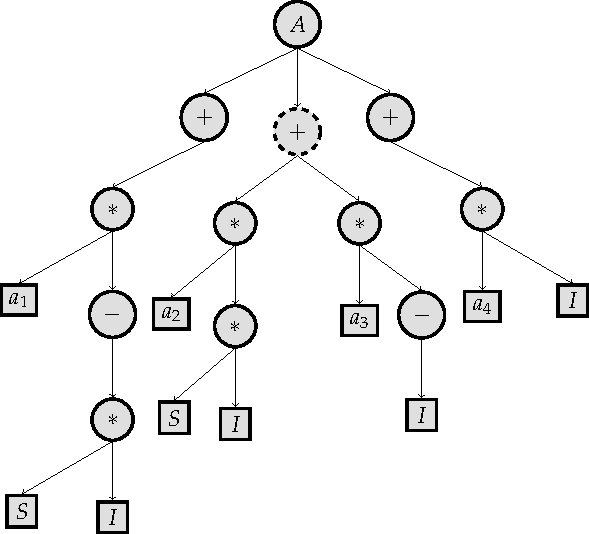
\includegraphics[width=0.47\textwidth]{"figures/cross_example_1.pdf"}
        \qquad
        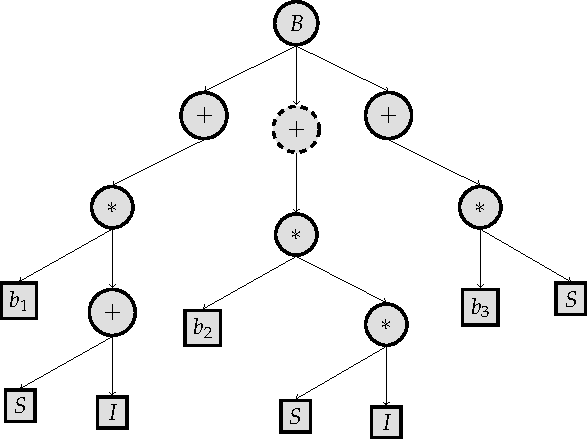
\includegraphics[width=0.47\textwidth]{"figures/cross_example_2.pdf"}
        \caption{Representación en forma de árboles de los sistemas A y B.}
        \label{tikzpicture:cross_example_1}
    \end{figure}
\end{center}
% \begin{center}
%     \begin{adjustbox}{width=0.5\textwidth, keepaspectratio}
%         \begin{tikzpicture}[
%                 roundnode/.style={circle, draw, fill=gray!25, very thick, minimum size=7mm},
%                 squarednode/.style={rectangle, draw, fill=gray!25, very thick, minimum size=5mm},
%                 roundnode_dashed/.style={circle, draw, dashed, fill=gray!25, very thick, minimum size=7mm},
%             ]
%             % Nodes
%             \node[roundnode]        (system)                            {$B$};

%             \node[roundnode]        (plus_S)     [below left=of system]        {$+$};
%             \node[roundnode]        (star_S_1)    [below left=of plus_S]    {$*$};
%             \node[squarednode]      (alpha_star_S_1)      [below left=of star_S_1]    {$b_1$};
%             \node[roundnode]        (add_S_2)    [below=of star_S_1]    {$+$};
%             \node[squarednode]      (S_star_S)       [below left=of add_S_2]   {$S$};
%             \node[squarednode]      (I_star_S)      [below=of add_S_2]   {$I$};

%             \node[roundnode_dashed]        (plus_I)     [below=of system]        {$+$};
%             \node[roundnode]        (star_I_1)    [below=of plus_I]    {$*$};
%             \node[squarednode]      (alpha_star_I_1)      [below left=of star_I_1]    {$b_2$};
%             \node[roundnode]        (star_I_2)    [below right=of star_I_1]    {$*$};
%             \node[squarednode]      (S_star_I)       [below left=of star_I_2]   {$S$};
%             \node[squarednode]      (I_star_I_1)      [below=of star_I_2]   {$I$};

%             \node[roundnode]        (plus_R)     [below right=of system]        {$+$};
%             \node[roundnode]        (star_R_1)    [below right=of plus_R]    {$*$};
%             \node[squarednode]      (beta_star_R_1)      [below=of star_R_1]    {$b_3$};
%             \node[squarednode]      (S_star_R)      [below right=of star_R_1]   {$S$};

%             %Lines
%             \draw [->] (system.south) -- (plus_S.north);
%             \draw[->] (system.south) -- (plus_I.north);
%             \draw[->] (system.south) -- (plus_R.north);

%             \draw[->] (plus_S.south) -- (star_S_1.north);
%             \draw[->] (star_S_1.south) -- (alpha_star_S_1.north);
%             \draw[->] (star_S_1.south) -- (add_S_2.north);
%             \draw[->] (add_S_2.south) -- (S_star_S.north);
%             \draw[->] (add_S_2.south) -- (I_star_S.north);

%             \draw[->] (plus_I.south) -- (star_I_1.north);
%             \draw[->] (star_I_1.south) -- (alpha_star_I_1.north);
%             \draw[->] (star_I_1.south) -- (star_I_2.north);
%             \draw[->] (star_I_2.south) -- (S_star_I.north);
%             \draw[->] (star_I_2.south) -- (I_star_I_1.north);

%             \draw[->] (plus_R.south) -- (star_R_1.north);
%             \draw[->] (star_R_1.south) -- (beta_star_R_1.north);
%             \draw[->] (star_R_1.south) -- (S_star_R.north);
%         \end{tikzpicture}
%     \end{adjustbox}
% \end{center}
y como resultado de la operación de cruzamiento se seleccionan los nodos que se resaltan con líneas discontinuas en la figura \ref{tikzpicture:cross_example_1}, entonces el sistema resultante $C$ sería:
\begin{align*}
    S' & = - a_1 * S * I \\
    I' & = b_2 * S * I   \\
    R' & = a_4 * I,
\end{align*}
que se representa con el árbol computacional que aparece en la figura \ref{tikzpicture:cross_example_2} de la página \pageref{tikzpicture:cross_example_2}.

\begin{center}
    % \begin{adjustbox}{width=0.5\textwidth, keepaspectratio}
    %     \begin{tikzpicture}[
    %             roundnode/.style={circle, draw, fill=gray!25, very thick, minimum size=7mm},
    %             squarednode/.style={rectangle, draw, fill=gray!25, very thick, minimum size=5mm},
    %             roundnode_dashed/.style={circle, draw, dashed, fill=gray!25, very thick, minimum size=7mm},
    %         ]
    %         % Nodes
    %         \node[roundnode]        (system)                            {$C$};

    %         \node[roundnode]        (plus_S)     [below left=of system]        {$+$};
    %         \node[roundnode]        (star_S_1)    [below left=of plus_S]    {$*$};
    %         \node[squarednode]      (alpha_star_S_1)      [below left=of star_S_1]    {$c_1$};
    %         \node[roundnode]        (neg_star_S_1)    [below=of star_S_1]    {$-$};
    %         \node[roundnode]        (star_S_2)    [below=of neg_star_S_1]    {$*$};
    %         \node[squarednode]      (S_star_S)       [below left=of star_S_2]   {$S$};
    %         \node[squarednode]      (I_star_S)      [below=of star_S_2]   {$I$};

    %         \node[roundnode_dashed]        (plus_I)     [below=of system]        {$+$};
    %         \node[roundnode]        (star_I_1)    [below=of plus_I]    {$*$};
    %         \node[squarednode]      (alpha_star_I_1)      [below left=of star_I_1]    {$c_2$};
    %         \node[roundnode]        (star_I_2)    [below right=of star_I_1]    {$*$};
    %         \node[squarednode]      (S_star_I)       [below left=of star_I_2]   {$S$};
    %         \node[squarednode]      (I_star_I_1)      [below=of star_I_2]   {$I$};

    %         \node[roundnode]        (plus_R)     [below right=of system]        {$+$};
    %         \node[roundnode]        (star_R_1)    [below right=of plus_R]    {$*$};
    %         \node[squarednode]      (beta_star_R_1)      [below=of star_R_1]    {$c_3$};
    %         \node[squarednode]      (I_star_R)      [below right=of star_R_1]   {$I$};

    %         %Lines
    %         \draw [->] (system.south) -- (plus_S.north);
    %         \draw[->] (system.south) -- (plus_I.north);
    %         \draw[->] (system.south) -- (plus_R.north);

    %         \draw[->] (plus_S.south) -- (star_S_1.north);
    %         \draw[->] (star_S_1.south) -- (alpha_star_S_1.north);
    %         \draw[->] (star_S_1.south) -- (neg_star_S_1.north);
    %         \draw[->] (neg_star_S_1.south) -- (star_S_2.north);
    %         \draw[->] (star_S_2.south) -- (S_star_S.north);
    %         \draw[->] (star_S_2.south) -- (I_star_S.north);

    %         \draw[->] (plus_I.south) -- (star_I_1.north);
    %         \draw[->] (star_I_1.south) -- (alpha_star_I_1.north);
    %         \draw[->] (star_I_1.south) -- (star_I_2.north);
    %         \draw[->] (star_I_2.south) -- (S_star_I.north);
    %         \draw[->] (star_I_2.south) -- (I_star_I_1.north);

    %         \draw[->] (plus_R.south) -- (star_R_1.north);
    %         \draw[->] (star_R_1.south) -- (beta_star_R_1.north);
    %         \draw[->] (star_R_1.south) -- (I_star_R.north);
    %     \end{tikzpicture}
    % \end{adjustbox}
    \begin{figure}[H]
        \centering
        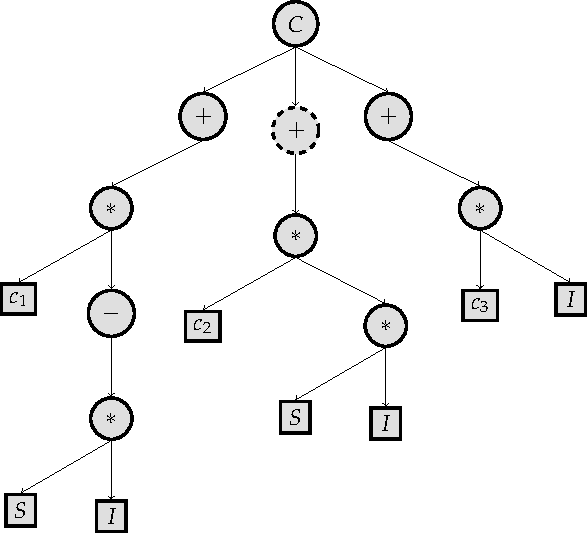
\includegraphics[width=0.6\textwidth]{"figures/cross_example_3.pdf"}
        \caption{Representación del resultado del cruzamiento entre los árboles A y B.}
        \label{tikzpicture:cross_example_2}
    \end{figure}
\end{center}

Una vez definidas las operaciones de mutación y cruzamiento solo faltaría detallar la operación de selección para tener totalmente definido el algoritmo genético. Los detalles de la última operación se presentan en la siguiente sección.

\section{Selección de las soluciones que pasan a la siguiente generación}\label{section:selection}

Dada una población inicial de $N$ individuos en una generación, se muta un subconjunto de individuos, y otro subconjunto se seleccionan para usar la operación de cruzamiento a partir de ellos. Al aplicar estas dos operaciones aparece un nuevo subconjunto de individuos. Este nuevo subconjunto se agrega a la población inicial de la generación, formando así un nuevo conjunto de individuos el cual se define como población total de la generación.

De la población total de la generación se seleccionan los $M$ individuos que mejor ajustan los datos. Se seleccionan también $N - M$ individuos aleatorios con el fin de evitar mínimos locales. Con estas dos selecciones se escoge de la población total de la generación una cantidad igual a la presente en la población inicial de la iteración. Los valores de $N$ y $M$ que se utilizaron durante los experimentos que aparecen en el capítulo \ref{chapter:results} son 100 y 10, respectivamente.

Como resultado de la selección se obtiene una nueva población que será la población de la siguiente generación. Las operaciones mutación, cruzamiento y selección se repiten un número fijo de veces que se define mediante el parámetro cantidad de generaciones. Esta repetición se realiza con el fin de generar varias iteraciones intentando obtener mejores soluciones cada vez.

En este capítulo se describió cómo representar, mediante árboles, un sistema de EDOs lineal con respecto a los parámetros, cómo calcular su costo para un conjunto de datos, así como la forma de cruzar y mutar estos sistemas. Con estos elementos se puede definir un algoritmo genético para determinar el sistema de EDOs lineal con respecto a los parámetros que mejor describa un conjunto de datos.

En el siguiente capítulo se muestran los resultados obtenidos de aplicar este algoritmo.